\documentclass[a4paper]{article}

\usepackage[english]{babel}
\usepackage[utf8]{inputenc}
\usepackage{amsmath}
\usepackage{graphicx}
\usepackage[colorinlistoftodos]{todonotes}
\usepackage[export]{adjustbox}[2011/08/13]
\usepackage{float}
\usepackage{bm}
\usepackage{hyperref}

\title{Behaviour Dynamics in Social Networks - Assignment 6}

\author{Maria Hotoiu, Federico Tavella}

\date{\today}

\begin{document}
\maketitle

\begin{abstract}
In this assignment the idea is to teach you how to work with social analysis software and data mining with social media data.
\end{abstract}

\section{Part A: Getting data from Social web media}

\subsection{Activity 1}

In the file \emph{home\_timeline.jsonl} there is my personal timeline (i.e. tweets about people that I am following) from Twitter and all the informations related to their profiles. I can retrieve my own tweets looking at the attribute \emph{screen\_name}. The code is parsing my timeline, obtaining informations and meta-data about the tweets contained in it and the related profiles.

Looking at the hashtags I can have an insight to events and locations related to the analyzed profile.

\subsection{Activity 2}

We chose the Twitter profile of Bill Gates because we thought that it could have had a large amount of different hashtags. It is interesting to find about that the  most common hashtags and words are referred to his commitment to defeat diseases such as polio and malaria through the Melinda and Bill Gates Foundation. It would be interesting to see the distribution of these tags over the time. In Figure~\ref{fig:term_distribution} and Figure~\ref{fig:hashtags_distribution} we can see, respectively, the distribution of the 1000 most used terms and hashtags.

\begin{figure}[!hbtp]
\centering
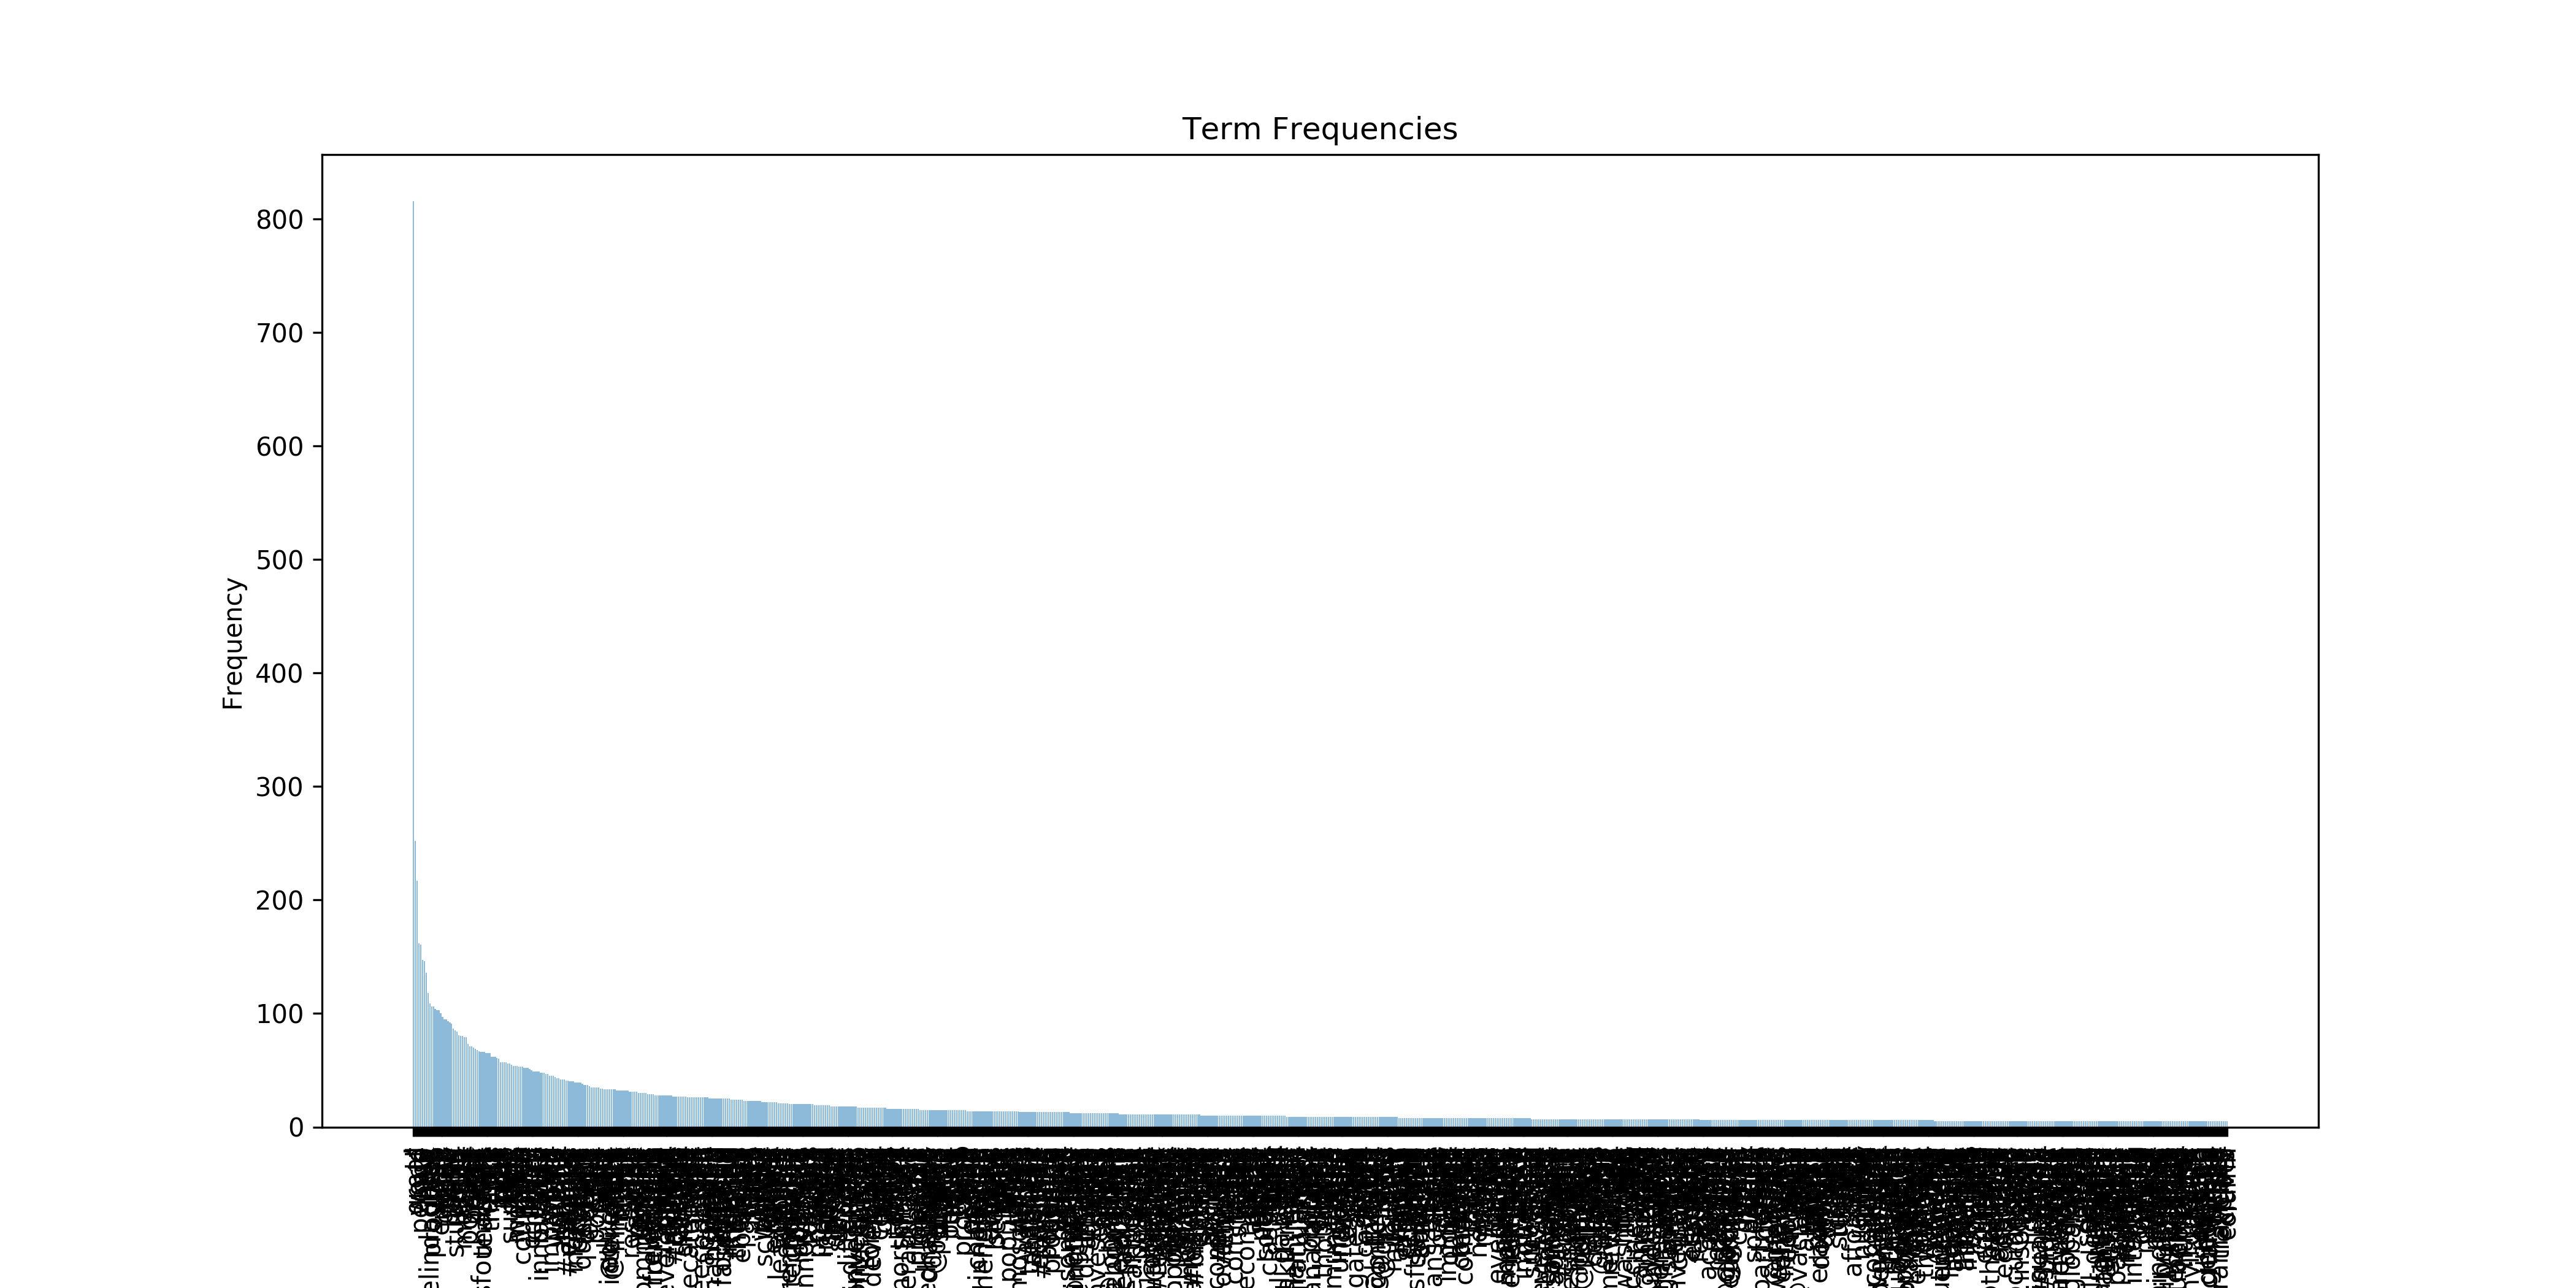
\includegraphics[width=\textwidth]{res/img/term_distribution}
\caption{Term distribution}
\label{fig:term_distribution}
\end{figure}

\begin{figure}[!hbtp]
\centering
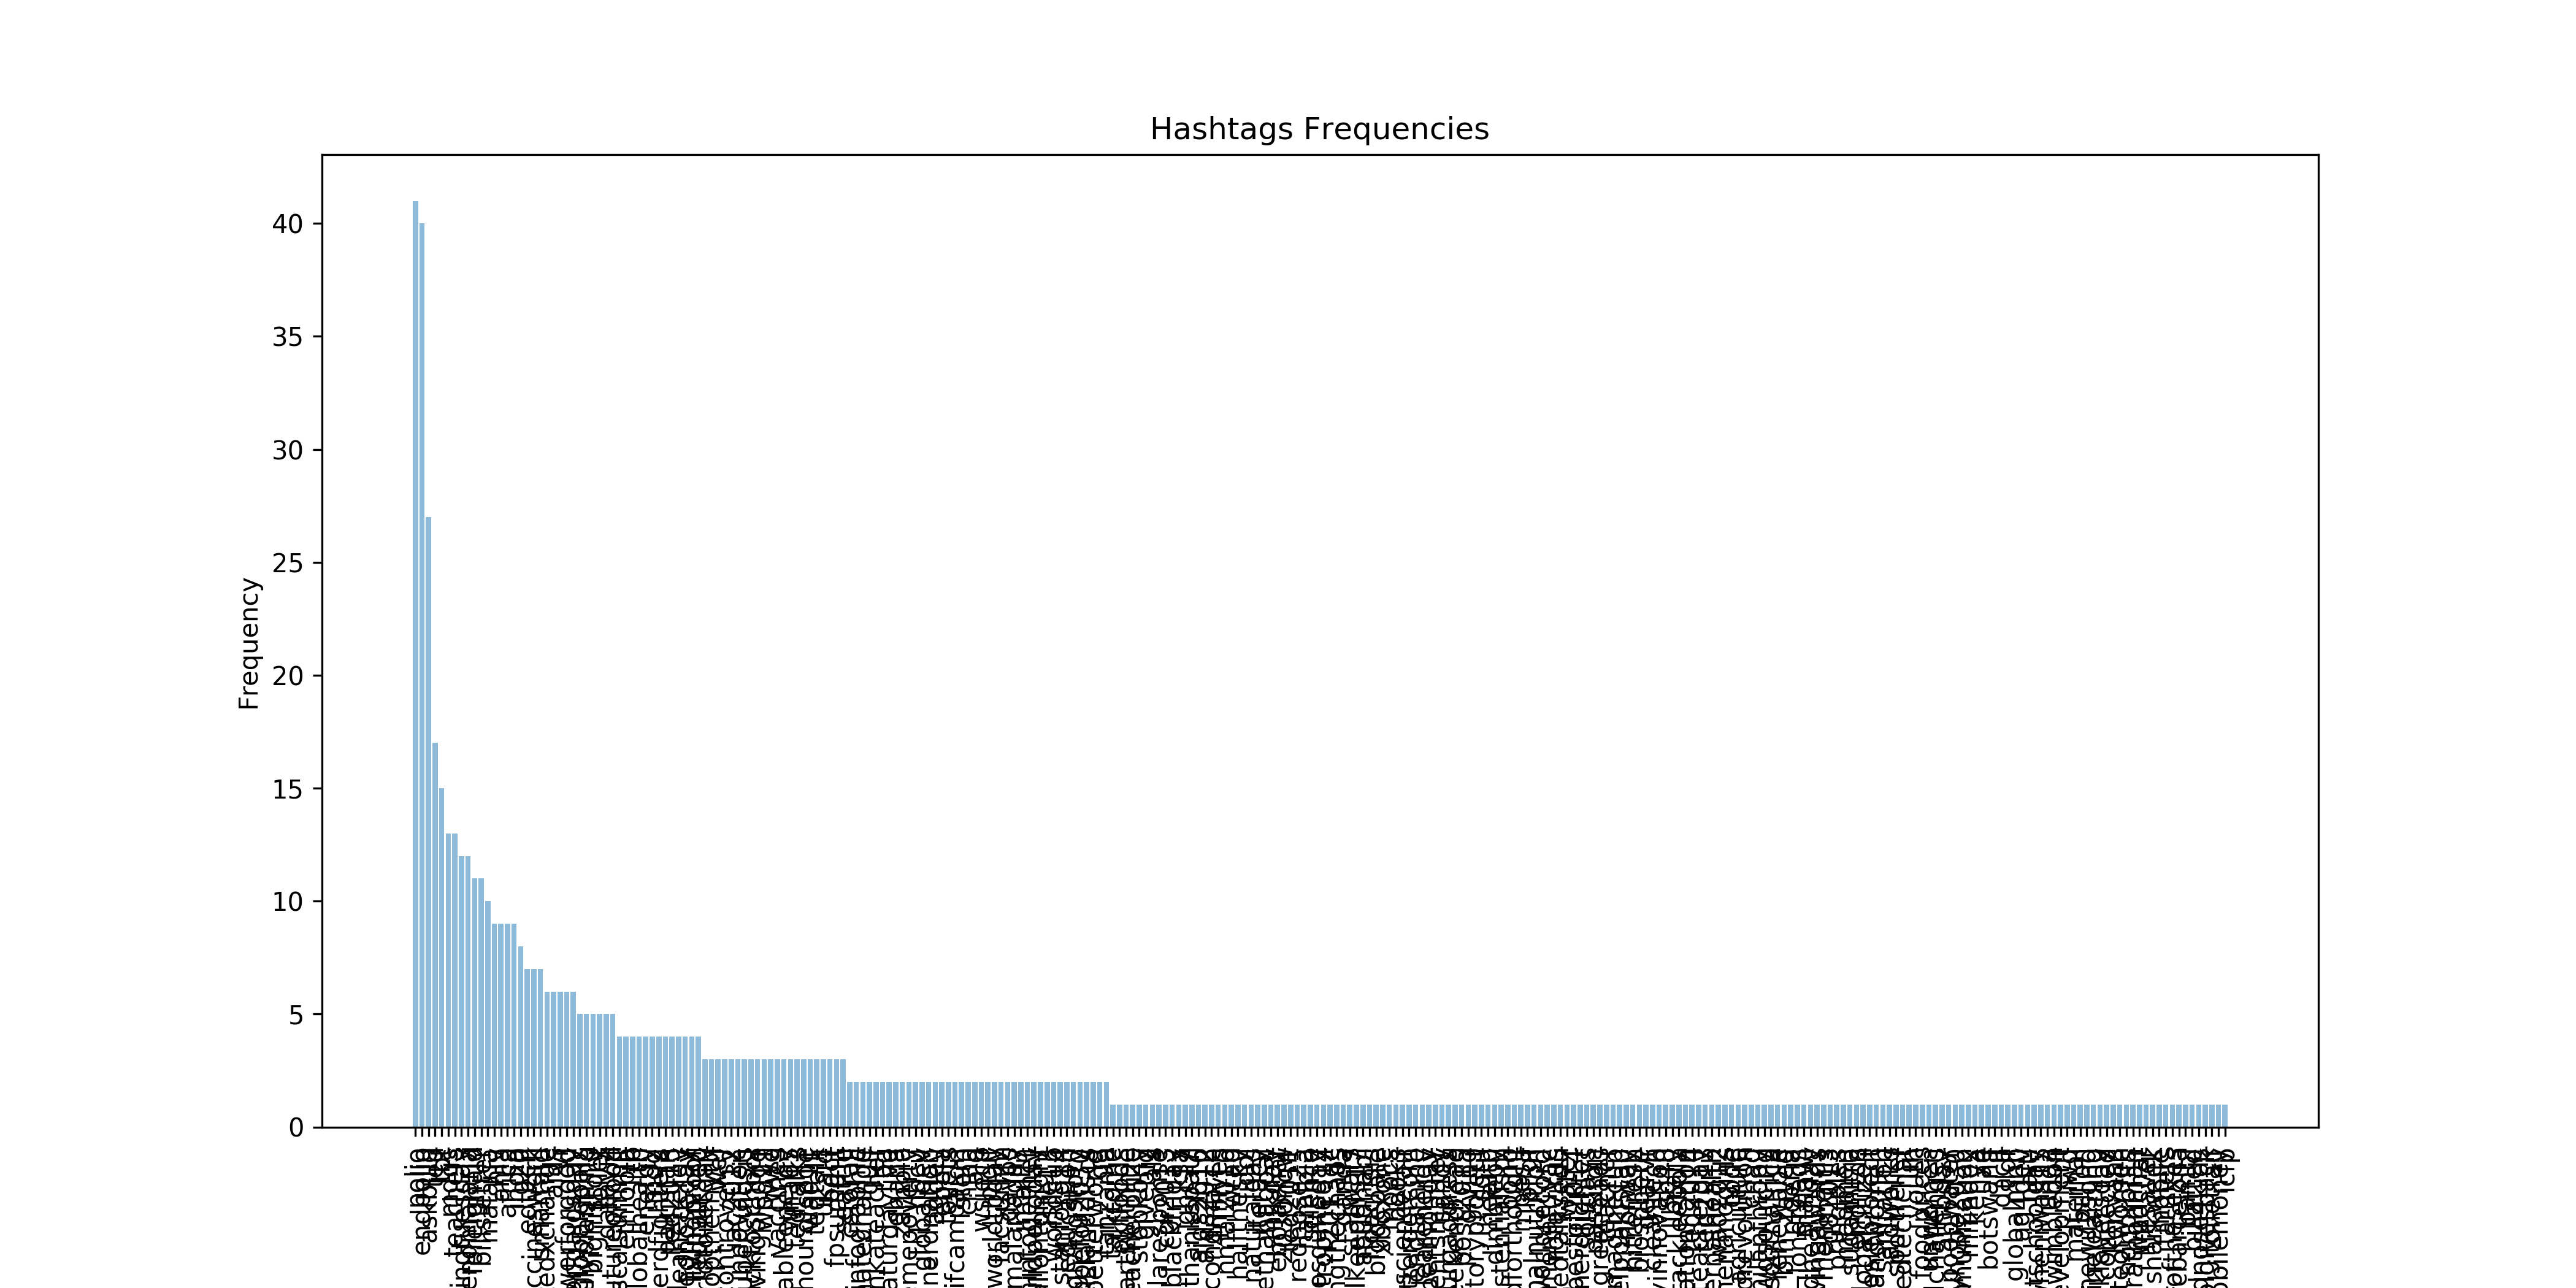
\includegraphics[width=\textwidth]{res/img/hashtags_distribution}
\caption{Hashtag distribution}
\label{fig:hashtags_distribution}
\end{figure}


\subsection{Activity 3}

My query is \emph{polio OR malaria}. Looking at the function \emph{CustomListener} and \emph{format\_filename} I can say that the results are going to be saved in a file named \emph{stream\_polio\_malaria.jsonl}.

\subsection{Activity 4}

Positive tweets (358):

\begin{enumerate}
\item RT @Lin\_Manuel: Gmorning! Happy \#GivingTuesday. If you don't have a dollar to give, you STILL have your time, your focus, your voice. Be g...
\item I'm amazed by how @NandanNilekani has lent his entrepreneurial passion to philanthropy. I'm delighted to welcome hi... \url{https://t.co/ly8PPvKz98}
\item I really enjoyed this conversation between our foundation CEO @SueDHellmann and Science Friday host @iraflatow. \url{https://t.co/xRfOtBumhg}
\item @johngreen Congrats @johngreen. I'm excited for you and your readers - including my daughter Phoebe, who's one of your biggest fans!
\item I always learn a lot from my friend @RayDalio. His new book \#Principles is a remarkable look at his life and career: \url{https://t.co/2A4EREQLYU}
\end{enumerate}

Negative tweets (32):

\begin{enumerate}
\item "The death that didn't happen is not visible. A fascinating conversation between @Atul\_Gawande and @Gladwell. \url{https://t.co/lLprByfc0u}
\item I'm very disappointed with today's decision to end \#DACA. Our statement: \url{https://t.co/67YQGYtDGo}
\item Melinda and I are deeply saddened to learn that our friend, mentor, and advisor Sam Dryden died this morning. \url{https://t.co/KnAhrA3Czh}
\item There has been incredible progress since the last Ebola outbreak. This is why we can't let up... \url{https://t.co/BWE2PG6ZFi}
\item 5/ I also have one big regret: When I left school, I knew little about the world's worst inequities. Took me decades to learn.
\end{enumerate}

We get this proportion of positive/negative tweets because the user (Bill Gates) tendentially tweets much more about positive aspects than negative ones. Probably, if he tweeted much more about negative things, he could have lost a lot of followers.

\section{Part B: Glasgow research on smoking habits in teenagers}

\subsection{Question 1}

If we chose $\Delta$t=1 year we would not be able to observe the relationships which involve people that were not yet part of the school cohort, or had already left the school cohort at one of the yearly points. 
$\Delta$t=5 would also not be a good choice because the total time (3 years) can not be divided into 5 months slots. 

\subsection{Question 2}

We chose time=6, so that the values of the states and the connection weights will be calculated for 6 consecutive time points, as if they were reviewed once every six months in the three years.\\
$\Delta$t=0.5 since we want to make measurements every half year.\\
The value chosen for the speed factor is 0.5. Since we are using the same speed factor for two different processes, its value should be as central between 0 and 1 as possible.


\subsection{Question 3}

The parameter choice depends on the problem we want to evaluate. The scenario based on which we chose the parameters is the one described in the answer of Question 2. 

\subsection{Question 4}
 
Changing the speed factor means changing how fast a connection between two people becomes stronger. A high speed factor means that the values of the connections will increase rapidly, while a lower speed factor means that the relationships will develop very slowly. 

The speed factor is also used to calculate how fast people who are connected to each other converge to the same smoking status. In this case, changing the speed factor means changing how fast people who are connected converge to the same smoking status.A high speed factor means fast convergence, while a low one means slow convergence. 

In therms of graphic modeling, a high speed factor is synonym with a steep graph, while a low speed factor is synonym with a flatter graph. 

\subsection{Question 5}

The amplification parameter is used to calculate the variation in the weights of the edges between two consecutive time points. This parameter dictates how big/small the change will be. A high amplification factor means a big change, while a low one means a small change. If we decrease the amplification factor, the difference between the weights of an edge at two consecutive time points will become smaller, meaning that the connection will strengthen slower. 

\subsection{Question 6}

In the real world, different processes happen with different speeds, so it would be reasonable to give different speed factors for the update of the edges and for the update of the states of the nodes. 
The processes we are modeling are interdependent, so changing the speed factor of one of them affects the other process as well. 

\subsection{Question 7}

In order to have a better representation of the graph, we also applied the Force Atlas 2 layout.

\begin{figure}[H]
\centering
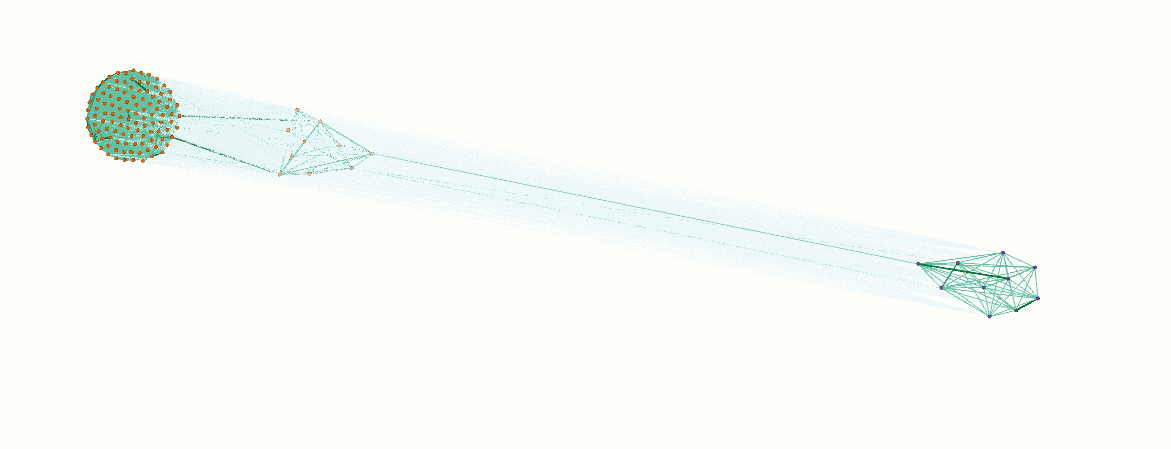
\includegraphics[width=\textwidth]{res/img/q17graph.png}
\caption{Graph resulted after Step 4}
\label{fig:network_output}
\end{figure}

\subsection{Question 8}

There are three clusters in our network, corresponding to the three levels of the smoking habit. The existence of these clusters illustrates the homophily principle.

\subsection{Question 9}
In the initial network, there are no clusters. The clusters are formed after applying the homophily principle. 

\subsection{Question 10}

In our network, the bridge between the two clusters disappears after applying the edge weight filter for weights bigger than 0.8.

\begin{figure}[H]
\centering
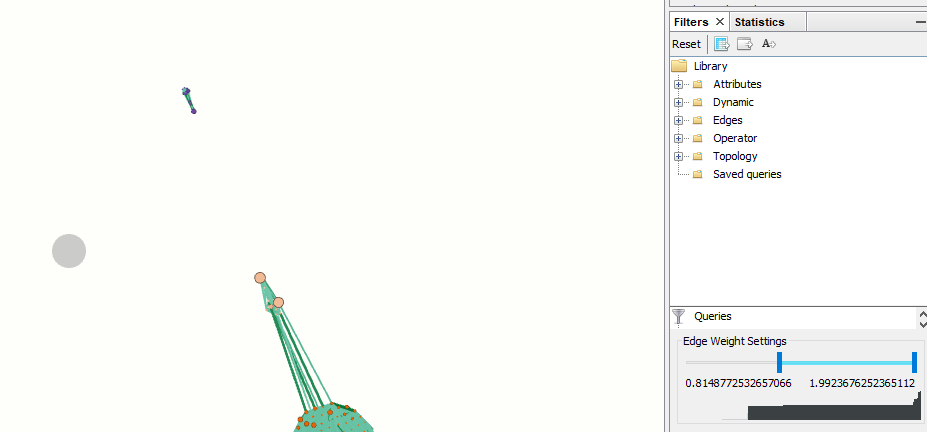
\includegraphics[width=\textwidth]{res/img/bridge.png}
\caption{The graph broken in two parts}
\label{fig:network_output}
\end{figure}

\end{document}
